\documentclass{article}

%%%%%%% PACKAGES %%%%%%%%
\usepackage[utf8]{inputenc}
\usepackage[margin=2cm]{geometry}
\usepackage{blindtext}
\usepackage{setspace}
\usepackage{graphicx}
\usepackage{notoccite} %citation number ordering
\usepackage{lscape} %landscape table
\usepackage{caption} %add a newline in the table caption
\usepackage{color}
\usepackage[dvipsnames]{xcolor}
\definecolor{ultramarine}{HTML}{2f3973}
\definecolor{hexablack}{HTML}{000000}
\usepackage[colorlinks = true,
linkcolor = hexablack,
urlcolor  = ultramarine,
citecolor = ultramarine,
anchorcolor = hexablack]{hyperref}

\usepackage[
backend=biber,  %references format (IEEE)
style=ieee,
sorting=none
]{biblatex}
\addbibresource{refs.bib} %rename this to your own bibliography
\onehalfspace   % 1.5 line spacing

\title{\huge{\textbf{Repota}} \\
\LARGE{A Service Report Application}}
\author{John Shields}
\date{February 2021}

\begin{document}
\pagenumbering{roman} % Start roman numbering
\clearpage\maketitle
\thispagestyle{empty}
\begin{center}
    \begin{figure}[h]
        \centering
        
\includegraphics[width=15cm]{images/logo-gmit.png}
        %\caption{Your caption here}
        \label{fig:logo}
    \end{figure}
    \textbf{Department of Computer Science and Applied Physics Galway-Mayo Institute of Technology}\\
    B.S.c. (Hons) in Software Development
    \bigskip
    \\ Applied Project and Minor Dissertation \\
    \textbf{Advised by: Andrew Beatty}
    
\end{center}
\newpage
\setcounter{page}{1}
\tableofcontents
\listoffigures

\newpage
\pagenumbering{arabic} % Start roman numbering

%%% CONTENT START HERE %%%%
\section{Introduction}

\subsection{GitHub Repository URLs}
\begin{itemize}
    % Dissertation Repository
    \item Project Dissertation: \url{https://github.com/johnshields/AP-MD-FYP/tree/main/dissertation} 
     % Application Repository
    \item Repota Application: \url{https://github.com/johnshields/Repota-App/tree/main/Repota}
    % Back-end Server Repository
    \item Horton Back-end Server: \url{https://github.com/johnshields/Repota-App/tree/main/horton} 
    % Database Repository
    \item Repota's Database: \url{https://github.com/johnshields/Repota-App/tree/main/database} 
\end{itemize}


\subsection{Project Introduction}
This project aimed to develop a service report application titled 'Repota' that relied on modern-day frameworks and technologies. The project focused on using these frameworks and technologies to build an app designed for automobile technicians to fill out service reports for auto dealerships and rental companies. The reports are done in a step by step process. Technicians can not only create their reports. They can view, edit, delete and export them to a PDF. These reports are usually done on paper or excel. Some similar apps have a similar idea, but it is almost as if they are trying to do too much for what they are supposed to be. With that said, there is no app that does just this service. This app is a necessity for technicians for their day-to-day work.
\\\\\ This project aimed to create a  sophisticated front-end framework to a quick back-end that would be connected to a stable and strong database. These technologies choices that were researched and implemented are as follows: Angular and Ionic for the front-end, Golang for the back-end and MySQL for the database. The back-end and database are hosted from a Linux Ubuntu Server. Before this project, Golang (Go) and a Linux Ubuntu Server were utterly new. Go's first version being released in 2012, meaning it is a relatively new language. 

\\\\\ \\\\
- write about the final product and how it came to be... 
\newpage

\begin{figure}[h!]
    \caption{Application Icon} % app logo
    \label{image:repotaChatLogo}
    \centering
    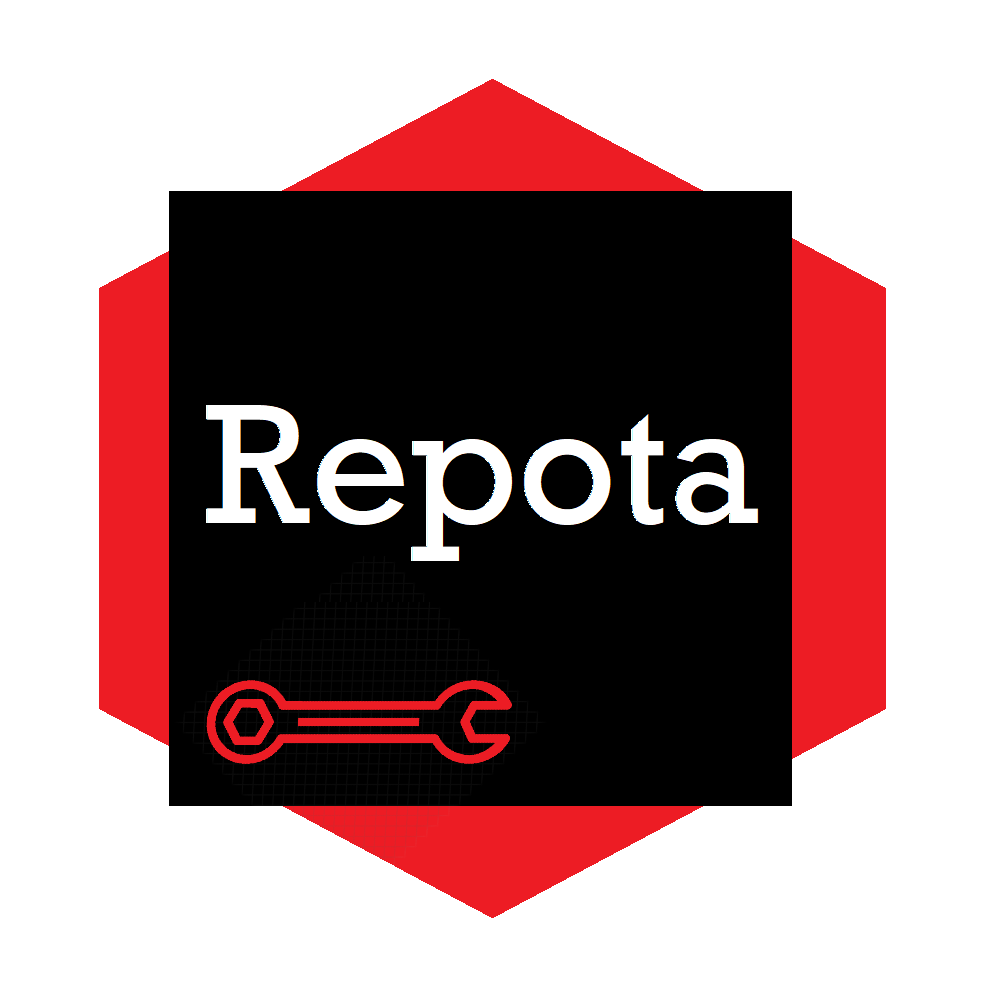
\includegraphics[width=0.6\textwidth]{images/repotaApp_logo.png}
\end{figure}

\newpage
\section{Methodology}
\subsection{Project Scope \& Goal}
The project scope had to have something along the lines of a system with several functioning parts that worked with as many new technologies as possible. Original ideas for this project where initially the likes of Desktop Application Development and Game Development. These possible routes for the projected were researched with the focus of on User Interface and experience. One of these ideas was a desktop application for people to send curriculum vitaes (CV) to companies that their CV related to. On the app the user would upload their CV. That CV would be then sent through a system that would read it, pick out the keywords, and send it to companies looking for future employees in that field. At first, this was a great concept, but constructing an app for with was an extensive scope as it would have to have either a vast database or some API to get/pull all these companies from different sources. 
\\\\ Another initial idea was to develop a fully-fledged Open World Game in Unity. This idea was drastically different from the others. Old noir films and parallel universes inspired the game. Making a mix of these two genres was quite exciting and meant that this open-world would have to be huge. This idea was a favorite. Unfortunately, it had to be forfeited as this project was to be done alone. This did not seem to be achievable as many more people (a full team) would be needed to develop a game of this size. If one person were to develop a game of this size, they would need a lot more time than is allocated for the project, especially balancing it with other modules.
\\\\ The chosen idea was settled to be a Service Report Web Application. This app was originally focused on being just a desktop app, but it was believed that this app would be very suitable to work on a tablet, so a mobile phone. So, therefore, the Ionic and Angular framework was chosen for the front-end. The app needed to be trusted with work-related data. Therefore, the desktop app focus was not ideal as the app will not ask for permission to access data associated with privacy settings.
\\\\ This app would need a quick back-end, so many technologies such as Node.js, Python, Java and Golang were heavily looked into. The back-end was narrowed down to use Google's language Golang (Go). This language is relatively new compared to other languages and had not been covered in the course modules. This means there are not many libraries, meaning that there are only a number or ways to go about writing the code.  The uniqueness of Go's compiler is that it is written in Go. Obviously, the very first compiler was not written in Go it was written in C. Go is capable of processing big files in seconds. It has been tested that Go is able to extract logs from a log file is around 25 seconds. This seemed to be the ideal back-end. Therefore it was chosen.
\\ A reliable and stable database was essential as this project purpose was to be used in a working environment meaning it would have to store a large quantity of data that needed to be accessed quickly and be able to add and update the data freely. MySQL was chosen for the database as it is very known for these mentioned qualities. 

\section{Technology Review}

\section{System Design}

\section{System Evaluation}

\section{Conclusion}

\newpage





%%% CONTENT HERE END %%%%
\end{document}
\newpage
\setstretch{1}  %reduce bibliography line spacing
\printbibliography
\end{document}